%!TEX root = ../template.tex
%%%%%%%%%%%%%%%%%%%%%%%%%%%%%%%%%%%%%%%%%%%%%%%%%%%%%%%%%%%%%%%%%%%%
%% 3-Background_Work.tex
%% NOVA thesis document file
%%
%% Chapter with the background work that is not necessary state of the art stuff but necessary for the explanation of the work done chapter.
%%%%%%%%%%%%%%%%%%%%%%%%%%%%%%%%%%%%%%%%%%%%%%%%%%%%%%%%%%%%%%%%%%%%

\typeout{NT FILE 3-Background_Work.tex}%

\chapter{Background Work}
\label{cha:Background work}

\glsresetall

\section{Introduction}
\label{sec.3:Introduction}

Several concepts are required for a proper understanding of this thesis. Some of them have not yet been introduced in the state of the art presented in Chapter~\ref{cha:State of the art}. These include different methods for spacing agents on $\mathbb{S}^2$ (Section~\ref{sec.3:Fibonacci Lattice}), the Mellinger controller (\ref{sec.3:Mellinger controller}), Lyapunov theory (Section~\ref{sec.3:Lyapunov Stability and Lyapunov-Based Control}), and consensus algorithms(Section~\ref{sec.3:Consensus-Based Coordination}).  

The following sections do not aim to provide a comprehensive treatment of these topics, instead, they present the fundamental concepts and tools necessary to fully understand the work developed in Chapter~\ref{cha:Developed Work}.

\section{Agent spacing on the two-sphere} \label{sec.3:Agent spacing on the two-sphere}
In this section, several methods for distributing points on a manifold are discussed. The primary objective is to achieve the most uniform spacing possible between agents. Such uniformity allows for more efficient use of each agent's reachability set at any given time. In other words, minimizing overlap between the reachability regions of different agents maximizes the collective coverage and effectiveness of the multi-agent system. For simplicity the two-sphere or unit sphere will be the main manifold considered since the problem at hand is encircling a target, where $\mathbb{S}^2 = \{\mathbf{x} \in \mathbb{R}^3 : \|\mathbf{x}\|_2 = 1\}$ denotes the unit sphere. 

Four different methods will be discusses including, lattitude and longitude, fibonnaci sphere, thomson minimum energy sphere and poisson disk sampling.

The sections \ref{sec.3:Latitude and longitude} and \ref{sec.3:Fibonacci Lattice} are both heavly inspired and influenced by \cite{Latitude_Longitude_vs_fibonacci}.

\subsection{Latitude and Longitude} \label{sec.3:Latitude and longitude}

The latitude--longitude lattice consists of points located at the intersections of a grid of meridians and parallels, separated by equal angular increments in latitude and longitude. This arrangement is commonly referred to as the \emph{latitude--longitude grid} or the \emph{equal-angle grid}. Due to the convergence of meridians toward the poles, the density of points increases with latitude, resulting in significant anisotropy.

The total number of points, denoted by $P$, depends on the angular spacing $\delta$ between adjacent grid lines. If the sphere is divided into $k$ equal angular intervals in latitude, so that $\delta = 180^\circ / k$ with $k = 1, 2, \ldots$, then the total number of grid points is

\begin{equation}
    P = 2k(k - 1) + 2 .
\end{equation}

This expression accounts for the $2k$ meridians and the $k - 1$ parallels, along with the two poles. A further limitation of this approach is that the total number of agents is constrained by the parameter $k$, which restricts the set of achievable formations. For example, configurations involving 3, 4, or 5 agents, cannot be realized within this framework.

\subsection{Fibonacci Lattice}
\label{sec.3:Fibonacci Lattice}

The Fibonacci lattice is named after the Fibonacci ratios, which were discovered in ancient India \cite{fibonacci_history}. The construction is based on the Fibonacci sequence, in which each term from the third onward is the sum of the two preceding terms:
\[
0, 1, 1, 2, 3, 5, 8, 13, 21, \ldots
\]

Given two consecutive Fibonacci numbers $F_i$ and $F_{i+1}$, the Fibonacci ratio is defined as $F_{i+1}/F_i$. As first proved by Robert Simson in 1753 \cite{fibonacci_to_golden_ratio_1,fibonacci_to_golden_ratio_2}, this ratio converges rapidly, as $i \to \infty$, to the golden ratio
\begin{equation}
  \varphi = 1 + \varphi^{-1} = \frac{1 + \sqrt{5}}{2} \simeq 1.618 .
  \label{eq:golden_ratio}
\end{equation}

The Fibonacci lattice differs from other spiral lattices on the sphere in that the longitudinal rotation between consecutive points along the generating spiral is the \emph{golden angle},
\begin{equation*}
  360^\circ \left(1 - \varphi^{-1}\right)
  = 360^\circ \varphi^{-2}
  \simeq 137.5^\circ ,
\end{equation*}
or, equivalently, its complementary angle,
\begin{equation*}
  360^\circ \varphi^{-1} \simeq 222.5^\circ .
\end{equation*}

In some lattice constructions, the golden ratio $\varphi$ is replaced by a rational approximant given by a Fibonacci ratio; this is the case when the total number of points is constrained to be a Fibonacci number. The golden angle optimizes packing efficiency in spiral lattices because the golden ratio is the \emph{most irrational} number, thereby avoiding periodic or near-periodic alignments in the spiral structure. As a result, lattice points do not cluster, and spatial uniformity is preserved.

When a Fibonacci ratio is employed, the total number of lattice points is $F + 1$, where $F > 1$ is a Fibonacci number. In contrast, the lattice used in this work is based directly on the golden ratio and admits any odd number of points.

To construct the lattice, let $N$ be a natural number and let the integer index $i$ range from $-N$ to $+N$. The total number of points is
\begin{equation}
P = 2N + 1 
\end{equation}

This forces the number of agents/points to always be odd.

The spherical coordinates (in radians) of the $i$th point are given by
\begin{align}
\text{lat}_i &= \arcsin\!\left(\frac{2i}{2N + 1}\right), \\
\text{lon}_i &= 2\pi i \varphi^{-1} .
\label{eq:fibonacci_lat_lon}
\end{align}

Each point is assigned a unique latitude, while the longitudinal separation between consecutive points corresponds to the golden angle (or its complement), approximately $222.5^\circ$.

Although not an academic reference, the interactive visualization provided in \href{https://observablehq.com/@meetamit/fibonacci-lattices}{Fibonacci Lattices} offers an intuitive and informative illustration of the Fibonacci lattice structure.

\subsection{Thomson minimum energy sphere} \label{sec.3:Thomson minimum energy sphere}

In 1904, J. J. Thomson proposed a model for the atom in which electrons were thought to be evenly distributed within a positively charged sphere. In this model, each electron experiences repulsive forces from the others and is constrained to remain on the surface of the sphere. This concept led to what is now known as the Thomson problem, which seeks the arrangement of $N$ electrons on the surface of a unit sphere that minimizes their total electrostatic potential energy, given that they repel each other according to Coulomb's law. Thomson introduced this problem while developing his atomic model, later called the plum pudding model, reflecting the understanding that negatively charged electrons exist within a neutrally charged atom.\cite{thomson_min_energy_sphere}

The Thomson problem can be formulated mathematically as the minimization of the total Coulomb energy of $N$ point charges constrained to lie on the unit sphere. Let $\mathbf{x}_i \in \mathbb{R}^3$ denote the Cartesian coordinates of the $i$-th point on the sphere, such that $\|\mathbf{x}_i\|_2 = 1$ for all $i = 1, \dots, N$. The total electrostatic potential energy is given by

\begin{equation}
E(\mathbf{X}) = \sum_{i=1}^{N} \sum_{j=i+1}^{N} \frac{1}{\|\mathbf{x}_i - \mathbf{x}_j\|_2},
\end{equation}

where $\mathbf{X} = [\mathbf{x}_1^\top, \mathbf{x}_2^\top, \dots, \mathbf{x}_N^\top]^\top \in \mathbb{R}^{N \times 3}$ is the matrix of all point coordinates, and $\|\mathbf{x}_i - \mathbf{x}_j\|_2$ is the Euclidean distance between points $i$ and $j$. The goal of the Thomson problem is to find

\begin{equation}
\mathbf{X}^* = \arg \min_{\mathbf{X} \in (\mathbb{S}^2)^N} E(\mathbf{X}),
\end{equation}

\subsubsection{Numerical approach}

The implementation was made using a gradient-based iterative solver, using a continuous optimization approach with steps projected onto the tangent plane of the sphere at each point. The key steps are as follows:

\begin{enumerate}
    \item \textbf{Initialization:} Points are initialized randomly on the unit sphere by normalizing random Gaussian vectors:
    \begin{equation}
    \mathbf{x}_i \leftarrow \frac{\mathbf{r}_i}{\|\mathbf{r}_i\|_2}, \quad \mathbf{r}_i \sim \mathcal{N}(\mathbf{0}, \mathbf{I}_3).
    \end{equation}

    \item \textbf{Force computation:} The repulsive Coulomb force on each point is computed as
    \begin{equation}
    \mathbf{F}_i = \sum_{j \neq i} \frac{\mathbf{x}_i - \mathbf{x}_j}{\|\mathbf{x}_i - \mathbf{x}_j\|_2^3}.
    \end{equation}
    This force is then projected onto the tangent plane of the sphere at $\mathbf{x}_i$ to ensure that the points remain on the surface:
    \begin{equation}
    \mathbf{F}_i^{\text{tangent}} = \mathbf{F}_i - (\mathbf{F}_i \cdot \mathbf{x}_i)\, \mathbf{x}_i.
    \end{equation}

    \item \textbf{Adaptive step update:} Points are moved along the tangent force direction with an adaptive step size $\alpha$ that decreases with iteration count:
    \begin{equation}
    \mathbf{x}_i \leftarrow \frac{\mathbf{x}_i + \alpha \mathbf{F}_i^{\text{tangent}}}{\|\mathbf{x}_i + \alpha \mathbf{F}_i^{\text{tangent}}\|_2}.
    \end{equation}
    To prevent stagnation in local minima, a small random jitter may be added occasionally:
    \begin{equation}
    \mathbf{x}_i \leftarrow \frac{\mathbf{x}_i + \mathbf{J}_i}{\|\mathbf{x}_i + \mathbf{J}_i\|_2}, \quad \mathbf{J}_i \sim \mathcal{N}(\mathbf{0}, \sigma^2 \mathbf{I}_3), \ \sigma \ll 1.
    \end{equation}

    \item \textbf{Convergence:} The iteration continues until the maximum displacement of any point between iterations falls below a specified tolerance, i.e.,
    \begin{equation}
    \max_i \|\mathbf{x}_i^{(k+1)} - \mathbf{x}_i^{(k)}\|_2 < \text{Tol}.
    \end{equation}
\end{enumerate}

\subsection{Poisson Disk sampling} \label{sec.3:Poisson sampling disk}

Poisson disk sampling is a stochastic sampling technique that enforces a minimum distance between samples, producing distributions that are both random and well-spaced. Formally, a Poisson disk distribution is defined such that no two samples are closer than a user-defined distance \gls{d_min}. This property avoids clustering while preserving randomness, resulting in so-called \emph{blue noise} characteristics, which are highly desirable for a very isotropous distributing of agents.

Poisson disk samples are generated using the fast algorithm proposed by Bridson\cite{poisson_sampling_disk}. The method improves efficiency by restricting candidate samples to a neighborhood around existing points. A background grid is used to accelerate distance queries, with the cell size chosen as \( \gls{d_min} / \sqrt{n} \) in an \( n \)-dimensional domain, ensuring that each cell contains at most one sample.

The algorithm starts by placing an initial random sample in the domain and adding it to an active list. While this list is not empty, a sample is selected and up to \gls{P_k} candidate points are generated uniformly in the spherical annulus between radii \( r \) and \( 2r \). If a candidate is at least distance \gls{d_min} from all existing samples, it is accepted and added to the active list. If no valid candidate is found after \gls{P_k} attempts, the sample is removed from the active list.

Because each iteration either adds or removes a sample and the number of candidate attempts is bounded by a constant, the overall computational complexity of the algorithm is \( O(N) \), being \( N \) the total number of samples. A key advantage of this approach is that it generalizes naturally to arbitrary dimensions, making it well suited for multi-dimensional sampling problems.

For a desired fixed number of agents \gls{N_D}, a challenge arises because standard Poisson disk sampling does not guarantee an exact number of generated points. To address this limitation, a gradient-based iterative solver might be cable of adjusting minimum separation distance necessary to guarantee a desired number of agents. This refinement might enable the placement of exactly \gls{N_D} agents with approximately uniform spacing. Owing to its low computational cost, such an approach could be practical for real-time or large-scale deployments. However, it should be noted that this remains a conceptual approach and has neither been proven feasible nor experimentally validated during the development of this thesis.

Figure~\ref{fig.4:methods_points_on_sphere} compares the distributions obtained from Poisson disk sampling with other methods discussed in the next chapter, illustrating its effectiveness in producing well-spaced points on the sphere. Being the run time shown in Figure~\ref{fig.4:comparing_methods_box_shape}.

\section{Simplified RUAV model}
As shown in \cite{AlexandraGonalvesRodrigues2023} the complete \gls{RUAV} model is quite complex and non-linear so an approximation of the \gls{RUAV} model is used and since the objective is to control the \gls{RUAV} movements so it follows the target vehicle, the model for the NMPC was simplified. This is possible given that we have a non-linear controller that allows for the combined control of the complete system. This version of the RUAV model becomes simply 

\begin{equation*}
\begin{aligned}
    \dot{\gls{p_D}}   &= \gls{v_D} \qquad &
    \dot{\gls{phi_D}} &= \gls{omega_D}
\end{aligned}
\end{equation*}

\section{Mellinger Controller} \label{sec.3:Mellinger controller}
The nonlinear internal controller used in this work is the Mellinger controller, named after Daniel Mellinger and Vijay Kumar \cite{Mellinger2011}. This controller receives as inputs the desired position \gls{p_D_ref}, velocity \gls{v_D_ref}, and attitude \gls{a_D_ref} \cite{AlexandraGonalvesRodrigues2023, Crazyflie_mellinger}, and computes the required thrust commands for each motor of a quadrotor. 

Figure~\ref{fig.3:mellinger_controller_architecture} illustrates the architecture of the Mellinger controller. Since this controller has been extensively validated in the literature and its detailed design is not the focus of this thesis, no further discussion is provided here.

\begin{figure}
  \centering
  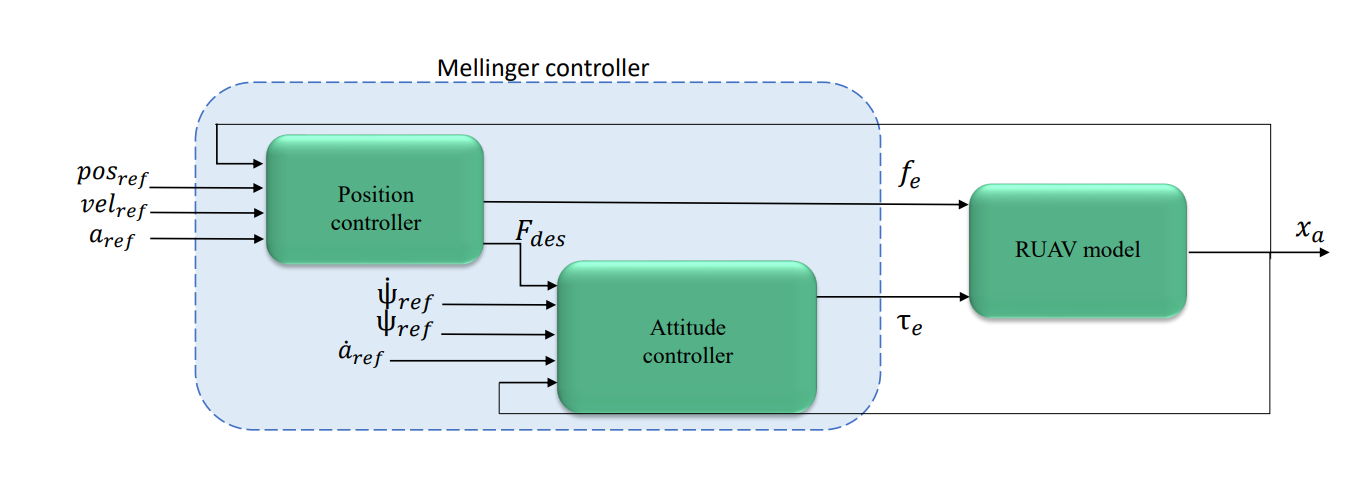
\includegraphics[width=\textwidth]{5-Figures/Chapter4/controller_architecture/mellinger_controller.png}
  \caption{Mellinger Controller [ROUBADO DA PATRÍCIA!! TENHO QUE FZR O MEU]}
  \label{fig.3:mellinger_controller_architecture}
\end{figure}

\section{Lyapunov Stability and Lyapunov-Based Control \textbf{[50\% CHAT GPT!!!]}} \label{sec.3:Lyapunov Stability and Lyapunov-Based Control}

Lyapunov theory provides a rigorous framework for analyzing the stability of nonlinear dynamical systems and for synthesizing stabilizing control laws without requiring explicit solutions of the system equations. In this work, Lyapunov-based methods are employed to analyze and guarantee the stability of a reduced-attitude control system evolving on nonlinear manifolds.

\subsection{System Description}

Consider a nonlinear dynamical system of the form
\begin{equation}
    \dot{\mathbf{x}} = \mathbf{f}(\mathbf{x}, \mathbf{u}),
\end{equation}
where $\mathbf{x} \in \mathbb{R}^n$ denotes the system state and $\mathbf{u} \in \mathbb{R}^m$ is the control input.  
An equilibrium point $\mathbf{x}_e$ satisfies $\mathbf{f}(\mathbf{x}_e, \mathbf{u}_e) = \mathbf{0}$ and can be shifted to the origin via an appropriate change of variables.

\subsection{Lyapunov Stability and Control}

Let $V : \mathbb{R}^n \rightarrow \mathbb{R}$ be a continuously differentiable, positive-definite function with $V(\mathbf{0}) = 0$.  
If its time derivative along system trajectories satisfies
\begin{equation}
    \dot{V}(\mathbf{x}) \le 0,
\end{equation}
then the equilibrium is Lyapunov stable. If $\dot{V}(\mathbf{x}) < 0$ for all $\mathbf{x} \neq \mathbf{0}$, asymptotic stability is ensured.

In Lyapunov-based control, the control law $\mathbf{u}(\mathbf{x})$ is designed such that the closed-loop dynamics yield a non-increasing Lyapunov function, guaranteeing stability by construction. This approach is particularly suitable for nonlinear systems evolving on manifolds, such as rigid-body attitude dynamics.

\subsection{Reduced Attitude Representation}

The attitude configuration of the rigid body is described by the unit vector
\begin{align}
q = Q e_3,
\end{align}
where \( Q \in SO(3) \) is the rotation matrix mapping vectors from the body frame \( I_b \) to the inertial frame \( I_R \), and \( e_3 = [0\;0\;1]^T \).
The configuration space is therefore the two-sphere
\begin{align}
S^2 = \left\{ q \in \mathbb{R}^3 \mid q^T q = 1 \right\}.
\end{align}

The kinematics of the reduced attitude evolve on \( S^2 \) according to
\begin{align}
\dot{q} = S(\omega) q,
\end{align}
where \( \omega \in \mathbb{R}^3 \) is the angular velocity expressed in the inertial frame and \( S(\cdot) \) denotes the skew-symmetric operator.

The rotational dynamics of the rigid body are given by
\begin{align}
J \dot{\omega} = u - c \omega - S(\omega) J \omega + \tau,
\end{align}
where \( J \) is the inertia matrix, \( c > 0 \) is a viscous damping coefficient, \( \tau \) represents external disturbances, and \( u \) is the control moment generated by the outer loop.

\subsection{Attitude Error Function on SO(2)}

Classical reduced attitude controllers frequently employ the error function
\begin{align}
\phi_r(q, q_d) = 1 - q^T q_d,
\qquad
e_r = S(q_d) q,
\end{align}
which exhibits degraded performance for large initial attitude errors, particularly when the relative angle exceeds \( \pi/2 \). In such cases, the magnitude of the error vector decreases as the misalignment increases, reducing the control authority and slowing convergence.

To address this limitation, an alternative error function inspired by \cite{lyapunov_outer_loop_control} is adopted:
\begin{align}
\phi_r(q, q_d) =
2 - \frac{2}{\sqrt{2}} \sqrt{1 + q^T q_d}.
\end{align}

This function is smooth and positive definite about \( q = q_d \), and avoids maximizing the error near the antipodal configuration. As a result, large-angle attitude errors are handled more effectively, as shown in Figure~\ref{fig.2:Comparison between error calculations}

% Subfigures 
\begin{figure}
\centering
\begin{subfigure}{.45\textwidth}
  \centering
  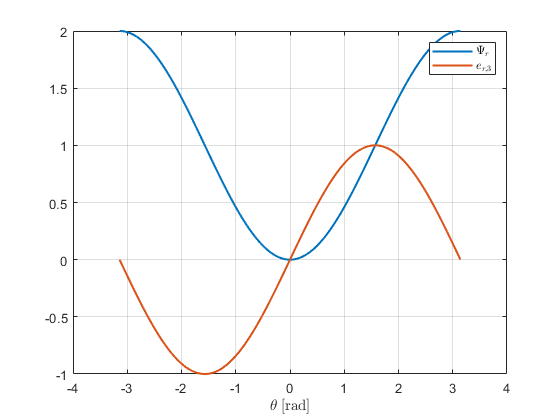
\includegraphics[width=\linewidth]{5-Figures/Chapter2/lyapunov/old_error.png}
  \caption{Standard method}
  \label{fig:sub1}
\end{subfigure}%
\begin{subfigure}{.45\textwidth}
  \centering
  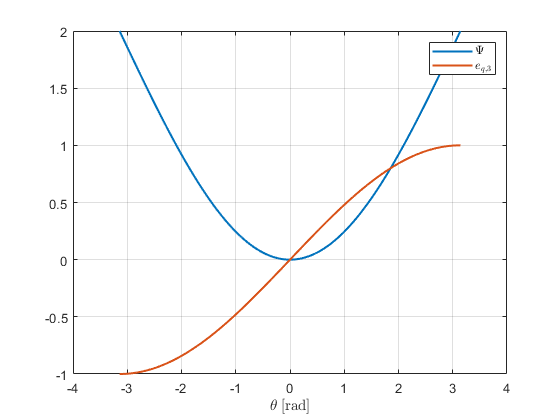
\includegraphics[width=\linewidth]{5-Figures/Chapter2/lyapunov/new_error.png}
  \caption{Proposed method in \cite{lyapunov_outer_loop_control}}
  \label{fig:sub2}
\end{subfigure}
\caption{Comparison between error calculations}
\label{fig.2:Comparison between error calculations}
\end{figure}

The corresponding configuration error vector is defined as
\begin{align}
e_q(q, q_d, Q) =
\frac{1}{\sqrt{2}\,\sqrt{1 + q^T q_d}}\,
Q^T S(q_d) q,
\end{align}
which lies in the tangent space \( T_q S^2 \).
This formulation ensures that the magnitude of the configuration error varies proportionally with the angular separation between \( q \) and \( q_d \), leading to uniform controller response across the sphere.

\subsection{Angular Velocity Error}

The angular velocity tracking error is defined by
\begin{align}
e_\omega = \omega - \omega_d,
\end{align}
where \( \omega_d \) is the desired angular velocity associated with the reference pointing direction \( q_d \).

\subsection{Control Law}

Using the above error definitions, the control moment is chosen as
\begin{align}
u =
Q^T\left(
- K_r Q e_q
- K_\omega e_\omega
\right)
+ S(\omega) J \omega
+ c \omega
- \tau,
\end{align}
where \( K_r \in \mathbb{R}^{3\times3} \) and \( K_\omega \in \mathbb{R}^{3\times3} \) are positive-definite gain matrices.

The first term stabilizes the configuration and angular velocity errors on \( S^2 \), while the remaining terms cancel the rigid-body nonlinearities, viscous damping, and external disturbances. This results in closed-loop error dynamics that are independent of the inertia matrix.

\subsection{Stability Properties}

Consider the Lyapunov candidate function
\begin{align}
V = \frac{1}{2} e_\omega^T J e_\omega + K_r \phi_r(q, q_d).
\end{align}

The time derivative of \( V \) along the closed-loop trajectories satisfies
\begin{align}
\dot{V} = - e_\omega^T K_\omega e_\omega \le 0,
\end{align}
showing that all system signals remain bounded and that the equilibrium
\(
(q,\omega) = (q_d,\omega_d)
\)
is asymptotically stable on \( S^2 \), excluding the antipodal configuration.

Importantly, the proposed error function eliminates the loss of control authority observed in classical formulations, resulting in improved convergence behavior for large initial attitude errors.

\subsection{Implementation and Simulation}

The proposed controller was implemented and evaluated through numerical simulations. The rigid body is initialized with a non-zero angular velocity and a large pointing error. A step change in the desired pointing direction is introduced during the simulation to evaluate transient performance.

The results in Figure~\ref{fig.2:lyapunov_example_results} demonstrate smooth convergence of the pointing direction on \( S^2 \), monotonic decrease of the attitude error function, and asymptotic regulation of the angular velocity. These results confirm the theoretical stability analysis and highlight the advantages of the proposed geometric formulation. A more extensive explanations and formula deduction can be found in the original referenced paper \cite{lyapunov_outer_loop_control}.

\begin{figure}[H]
\centering

\begin{minipage}{\textwidth}
\centering
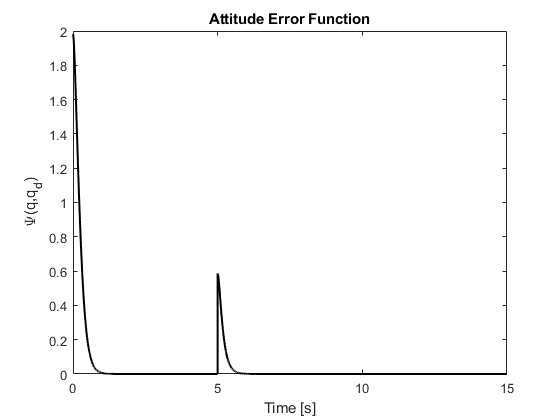
\includegraphics[width=0.45\textwidth]{5-Figures/Chapter2/lyapunov/Attitude_error.png}\hfill
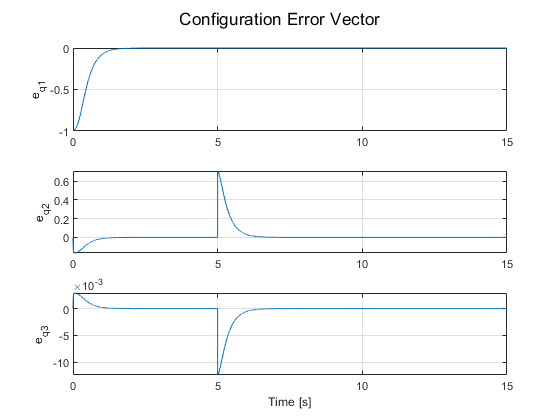
\includegraphics[width=0.45\textwidth]{5-Figures/Chapter2/lyapunov/configuration error vector.png}
\end{minipage}

\vspace{0.5cm}

\begin{minipage}{\textwidth}
\centering
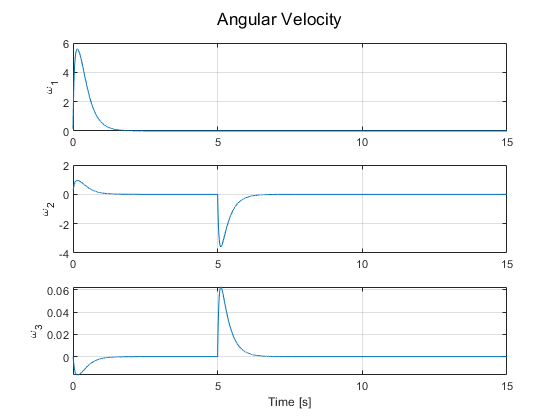
\includegraphics[width=0.45\textwidth]{5-Figures/Chapter2/lyapunov/angular velocity error.png}\hfill
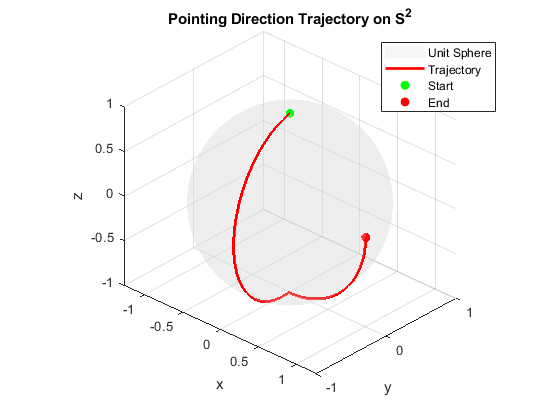
\includegraphics[width=0.45\textwidth]{5-Figures/Chapter2/lyapunov/traking trajectory.png}
\end{minipage}

\caption{Lyapunov example results}
\label{fig.2:lyapunov_example_results}
\end{figure}

\section{Consensus-Based Coordination  \textbf{[100\% CHAT GPT!!!]} \textbf{[MISSING CITATIONS]}} \label{sec.3:Consensus-Based Coordination}
\todo{This entire section}
Consensus-based coordination is a fundamental approach in multi-agent systems, where a group of agents cooperatively achieves a common objective through local interactions.
Typical applications include formation control, distributed estimation, flocking, and cooperative robotics.
The key idea is that global coordination emerges from simple local interaction rules defined by the communication network.

\subsection{Graph-Theoretic Representation}

The interaction topology of a multi-agent system is commonly modeled using graph theory.
Let the communication network be represented by a graph
\begin{equation}
    \mathcal{G} = (\mathcal{V}, \mathcal{E}),
\end{equation}
where $\mathcal{V} = \{1,2,\dots,N\}$ is the set of nodes (agents) and $\mathcal{E} \subseteq \mathcal{V} \times \mathcal{V}$ is the set of edges representing information exchange.

If information flow between agents is bidirectional, the graph is undirected; otherwise, it is directed.
The connectivity properties of $\mathcal{G}$ play a crucial role in determining whether consensus can be achieved.

\subsection{Adjacency Matrix}

The \textit{adjacency matrix} $\mathbf{A} \in \mathbb{R}^{N \times N}$ characterizes the local interactions among agents.
Its elements are defined as
\begin{equation}
    a_{ij} =
    \begin{cases}
        w_{ij} > 0, & \text{if agent $j$ sends information to agent $i$}, \\
        0, & \text{otherwise},
    \end{cases}
\end{equation}
where $w_{ij}$ denotes the weight of the communication link.
For undirected graphs, $\mathbf{A}$ is symmetric.

The adjacency matrix determines which agents influence each other and with what relative strength.
However, it does not explicitly capture the notion of disagreement between agents, which is central to consensus dynamics.

\subsection{Laplacian Matrix}

The \textit{graph Laplacian matrix} encodes both the adjacency structure and the degree of each node.
It is defined as
\begin{equation}
    \mathbf{L} = \mathbf{D} - \mathbf{A},
\end{equation}
where $\mathbf{D} = \text{diag}(d_1, \dots, d_N)$ is the degree matrix with
\begin{equation}
    d_i = \sum_{j=1}^{N} a_{ij}.
\end{equation}

The Laplacian matrix plays a central role in consensus analysis.
It has the following important properties:
\begin{itemize}
    \item $\mathbf{L}\mathbf{1} = \mathbf{0}$, where $\mathbf{1}$ is the vector of all ones.
    \item All eigenvalues of $\mathbf{L}$ are non-negative.
    \item The multiplicity of the zero eigenvalue equals the number of connected components of the graph.
\end{itemize}

For undirected and connected graphs, $\mathbf{L}$ has a single zero eigenvalue, which is a necessary and sufficient condition for consensus.

\subsection{Consensus Algorithms}

Consider a group of $N$ agents, each with scalar state $x_i \in \mathbb{R}$.
A standard continuous-time consensus protocol is given by
\begin{equation}
    \dot{x}_i = \sum_{j=1}^{N} a_{ij} (x_j - x_i),
\end{equation}
which can be written in compact form as
\begin{equation}
    \dot{\mathbf{x}} = -\mathbf{L}\mathbf{x}.
\end{equation}

This dynamics drives the agents toward a common value by reducing the disagreement between neighboring states.
If the communication graph is connected, all states converge to a consensus value
\begin{equation}
    \lim_{t \to \infty} x_i(t) = x^\ast, \quad \forall i.
\end{equation}

For undirected graphs, the consensus value corresponds to the average of the initial states.
The convergence rate is influenced by the second smallest eigenvalue of the Laplacian, known as the \textit{algebraic connectivity}.

\subsection{Extensions and Remarks}

Consensus algorithms can be extended to higher-order agent dynamics, time-varying topologies, directed graphs, and delayed communication.
Despite these complexities, the Laplacian matrix remains the fundamental tool for analyzing stability and convergence.
As a result, consensus-based coordination provides a scalable and fully distributed framework for multi-agent control systems.

\subsection{Summary}

Consensus-based coordination relies on local interactions defined by a communication graph to achieve global agreement.
The adjacency and Laplacian matrices provide compact representations of the network structure and are essential for the design and analysis of consensus algorithms.
Their spectral properties directly determine the existence, speed, and robustness of consensus.